\chapter{Grundlagen}

Ziel dieser Arbeit ist die Ermittlung optimierter Gebäudeenergiesysteme für den deutschen Wohngebäudebestand.
Hierzu wurde in Kapitel \ref{sec:Sektion 21} der Bestand analysiert, um auf dieser Untersuchung aufbauend die nationale Wohngebäudesituation in einigen wenigen, repräsentativen Klassen abzubilden. 
Des Weiteren wurde in \ref{sec:Sektion 22} die historische Entwicklung der deutschen Dämmstandards betrachtet. Daraus wurden Zeiträume der Baualtersklassen mit ähnlichen Wärmeübergangskoeffizienten der Gebäudehülle zusammengefasst. 
Zuletzt stellt Kapitel \ref{sec:Sektion 23} die Grundlagen der mathematischen Optimierung sowie das im Rahmen dieser Arbeit erweiterte Optimierungsprogramm vor. 

Die Gebäudeklassen sollen für die Bestimmung der Gebäudeenergiesysteme mit dem Optimierungsprogramm benutzt werden. 
Hieraus soll ein Vergleich zwischen Emissionsoptimum sowie Kostenoptimum gewonnen werden.

%Gebäudeenergiesysteme erklären?
%Was hat das überhaupt mit Grundlagen zu tuen, was ich da schreibe?
%Nehm ich in der Einleitung des Kapitels hier zuviel vorweg?
%Ist es okay, hier den Vergleich zu erwähnen? Evl. umschreiben
%Letzter Satz beschissen





\section{Deutscher Wohngebäudebestand}
\label{sec:Sektion 21}

Zunächst wurde der Wohngebäudebestand hinsichtlich Alter und Größe ausgewertet.
Als Daten wurden die Statistiken des Zensus2011, einer nationalen statistischen Erhebung von privaten Haushalten, betrachtet. 
Besagte Statistiken wurden in verschiedenen wissenschaftlichen Untersuchungen des Institut für Wohnen und Umwelt GmbH (IWU) ausgewertet und evaluiert.
Weiterhin wurde für die gebäudetypischen Kennwerte die Typgebäude des europaweiten TABULA Projekts berücksichtigt.
%Tabula evtl erst im nächsten Kapitel erläutern, da bei der statistischen Betrachtung fast nur Zensus/IWU Daten betrachtet werden

Nach den 2011 veröffentlichten Zensus Daten besteht der deutsche Wohngebäudebestand aus rund 18.368.000 Gebäuden mit 39.432.000 Wohnungen \cite{.2015}.
Wie in Abbildung \ref{fig: Abbildung211} zu erkennen ist, prägt den deutschen Wohngebäudebestand einen Boom in der Nachkriegszeit. 
So wurden in den Jahren von 1949 bis 1978 etwa 7,2 Millionen Häuser errichtet. Diese Klasse alleine macht \mbox{38 \%} der deutschen Wohngebäude aus. 
Mit ca. 2,7 Millionen Gebäuden und einem Anteil von etwa \mbox{14 \%} bilden die vor 1919 fertiggestellten Wohnobjekte den zweitgrößten Anteil, sowie die Häuser mit Baualter zwischen 1919 und 1948 mit knapp \mbox{12 \%} die drittgrößte Gruppe.
Folglich sind knapp zwei Drittel der deutschen Wohngebäude vor 1978 erbaut worden.
Eine weitere relevante Klasse beschreiben mit fast \mbox{10 \%} die von 1979 bis 1986 geschaffenen Wohnbauten. 
Zusammen mit den drei Klassen \mbox{1987 - 1990,} \mbox{1991 - 1995} und \mbox{1996 - 2000} werden  durch diese vier Gruppen mehr als ein Viertel des Wohngebäudebestandes in Deutschland abgebildet.
Im Gegensatz zu den zuvor genannten Gruppen stellen die nach der Jahrtausendwende konstruierten Häuser mit unter \mbox{10 \%} und nur 1,6 Millionen Häusern einen relativ kleinen Anteil des nationalen Bestandes dar. 

Es sei noch zu erwähnen, dass in dieser Betrachtung den Mikrozensus-Klassen gefolgt wurde. 
Diese sind explizit keine gleich langen Zeitintervalle, sondern \glqq orientieren sich an historischen Einschnitten, den Zeitpunkten statistischer Erhebungen und den Veränderungen der wärmetechnisch relevanten Bauvorschriften\grqq \cite{.2015}. 
So beschreibt beispielsweise das relativ kurze Zeitintervall von 1979 bis 1983 den Zeitraum zwischen erster und zweiter Wärmeschutzverordnung, auf welche in Kapitel \ref{sec:Sektion 22} noch näher eingegangen wird.

\begin{figure}[H]
	\centering
		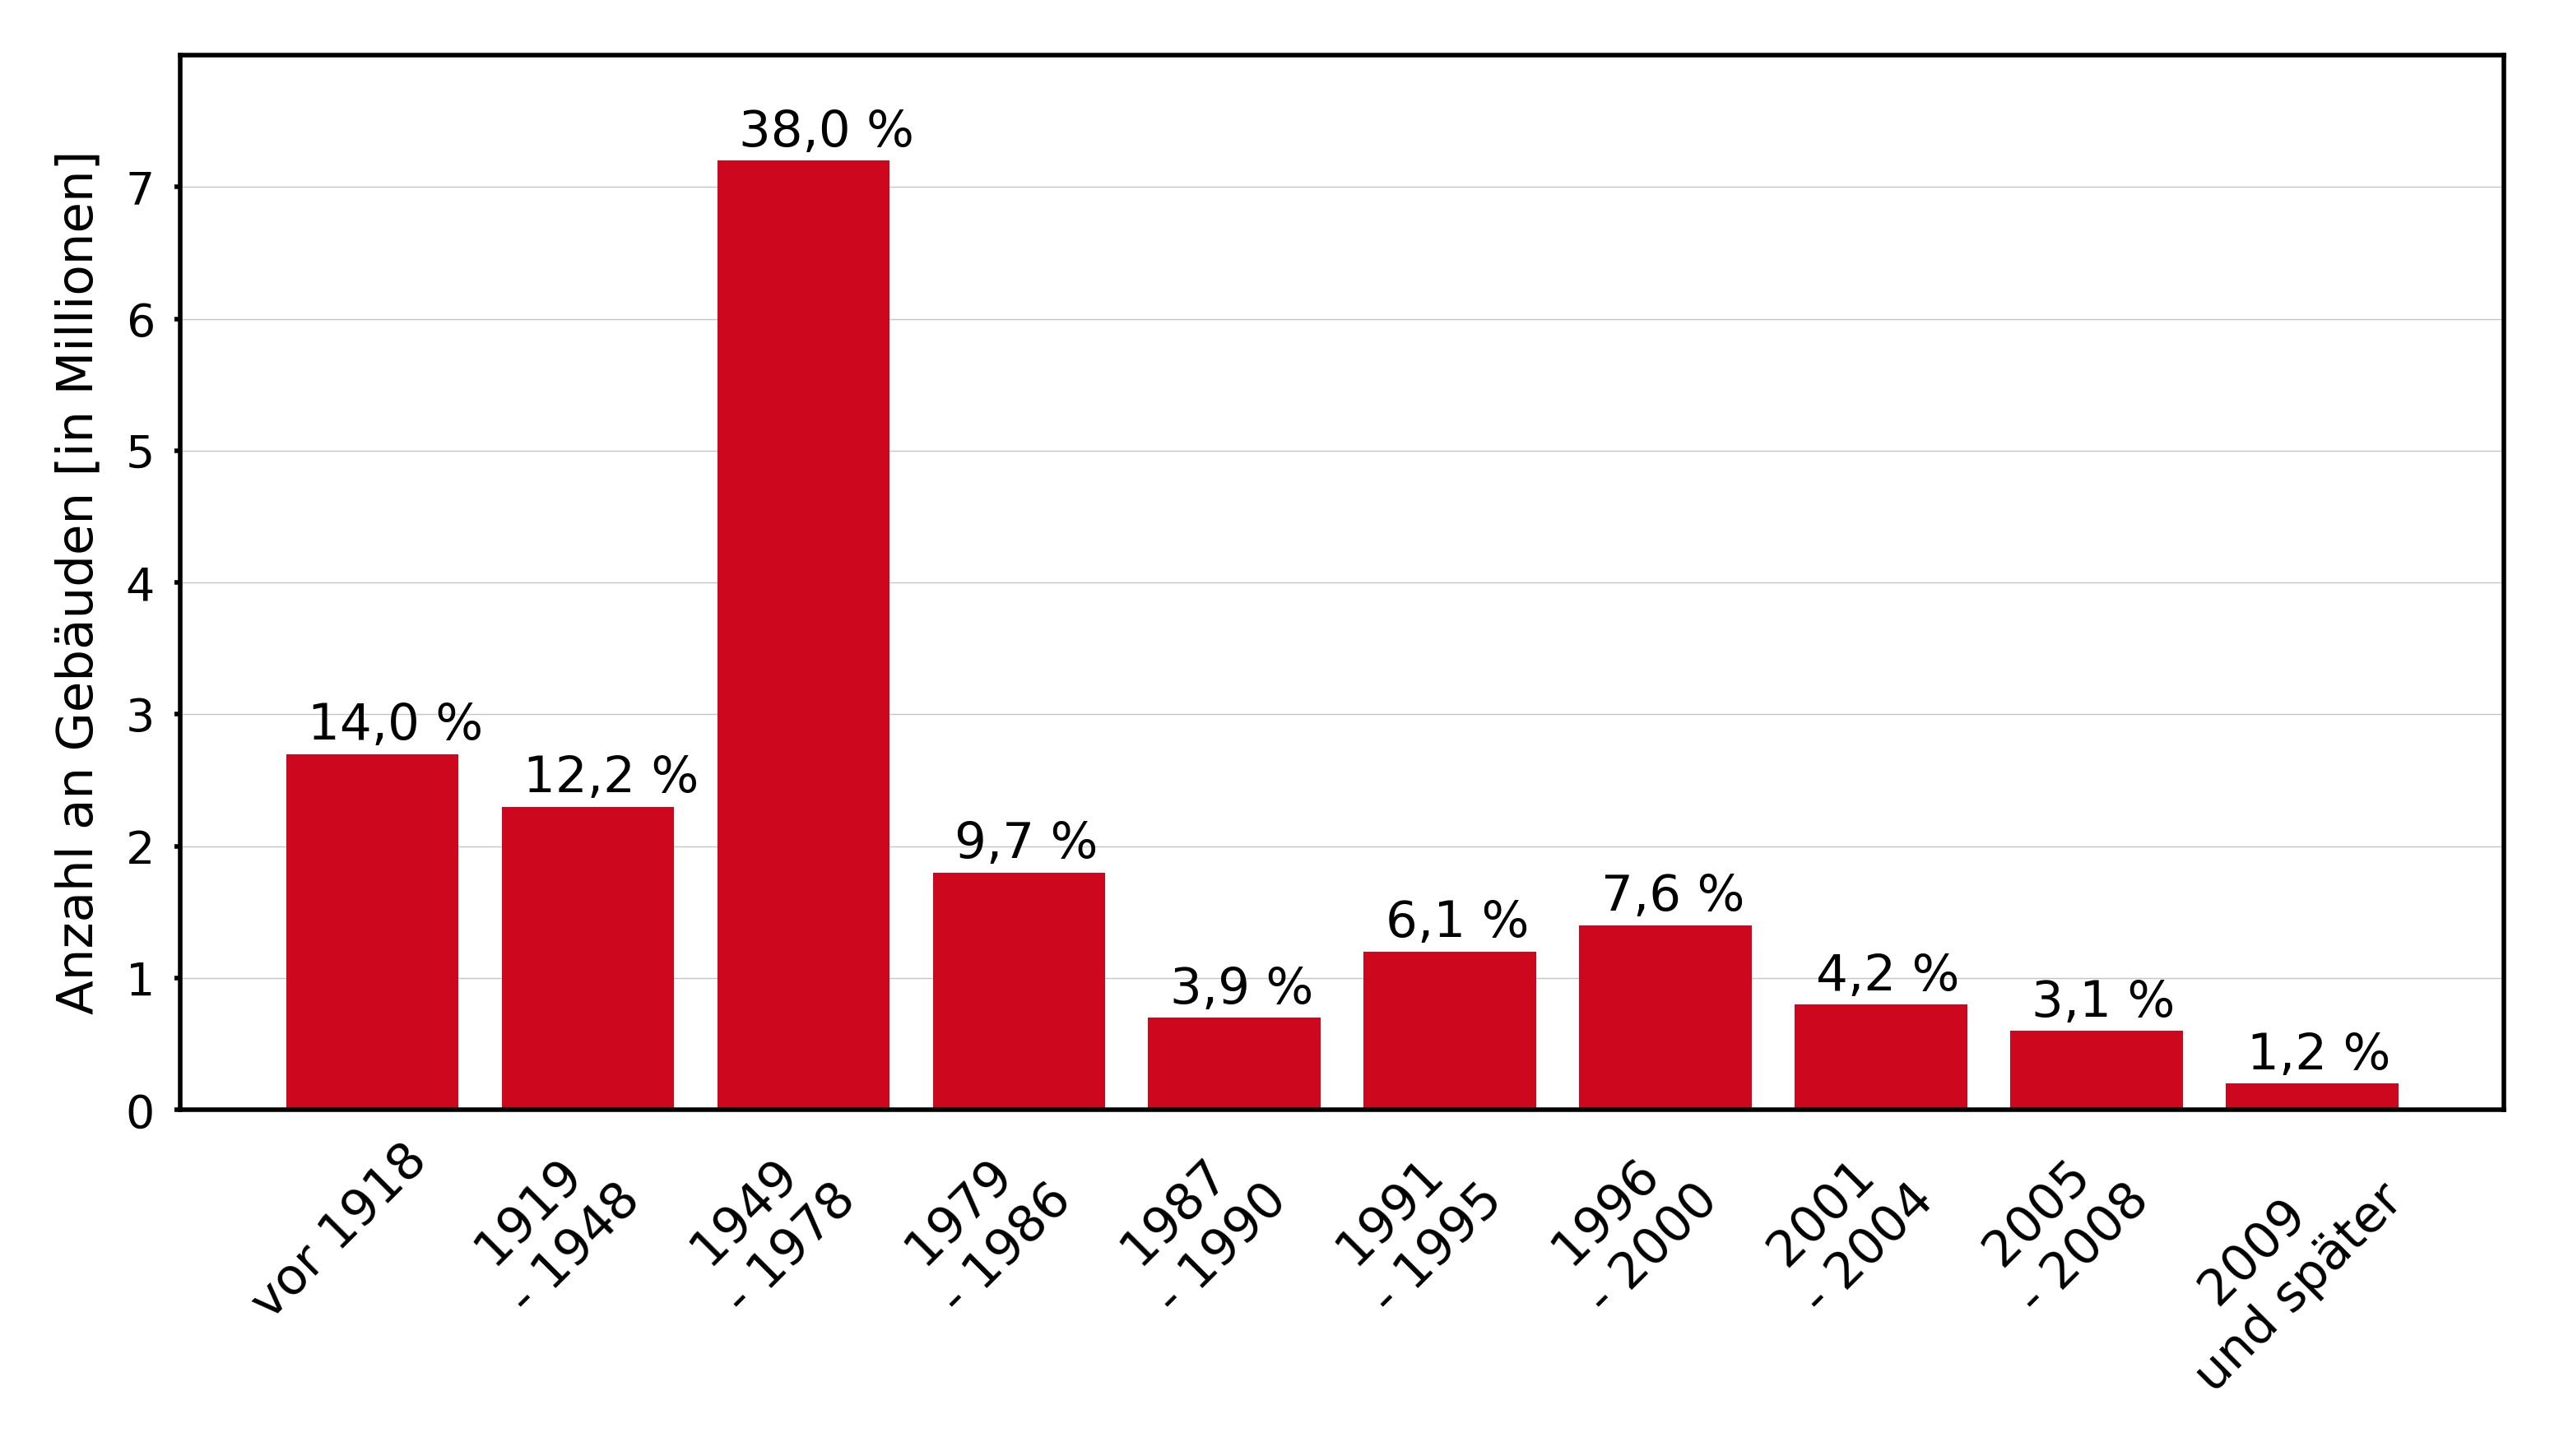
\includegraphics{Pictures/GebaeudeAlterDiagramm.jpg}
	\caption{errichtete Wohngebäude nach Mikrozensus-Klassen  	\cite{StatistischeAmterdesBundesundderLander.2014}}
	\label{fig: Abbildung211} 
\end{figure}
%Zwanzig Jahre Klassen vorstellen?

Eine weitere Unterteilung des Wohngebäudebestandes erhält man bei der Betrachtung der Anzahl an Wohneinheiten im Gebäude. 
Hierbei setzt sich der Bestand zu zwei Dritteln aus Wohngebäuden mit nur einer Wohnung zusammen. 
Weitere \mbox{17 \%} bilden Gebäude mit zwei Wohnungen und die Gebäudeklasse mit \mbox{3 - 6 Wohnungen} ist mit \mbox{12 \%} vertreten. 
Die größeren Gebäude mit \mbox{7 - 12 Wohnungen} sowie mit 13 und mehr Wohnungen sind anteilig am Gebäudebestand mit jeweils \mbox{5 \%} und \mbox{1 \%} relativ kleine Gruppen. 
Allerdings gelten letztere nur bei einer Gebäudebetrachtung als weniger relevant, da sie bei einer Anschauung der Wohneinheiten logischerweise mit größeren Faktoren eingehen. \cite{StatistischeAmterdesBundesundderLander.2014b}

In Abbildung \ref{fig: Abbildung212} sind die Anzahl der Wohneinheiten für die drei Baualtersklassen älter als 1978, \mbox{1979 - 1994} und \mbox{1995 - 2009} sowie deren Anteil an allen Wohneinheiten bis Baujahr 2009 des Gebäudebestandes dargestellt. 
In Anlehnung an den vorherigen Abschnitt werden Gebäude mit bis zu 2 Wohnungen als Einfamilienhäuser zusammengefasst und nach der englischen Bezeichnung \glqq single family home\grqq \,mit SFH abgekürzt. 
Wohngebäude mit 3 oder mehr Wohnungen werden als Mehrfamilienhäuser mit der Abkürzung MFH für \glqq multy family home\grqq\,gebündelt. 

Auffallend ist wiederum der enorme Anteil der Gebäude mit Baualter älter als 1978. 
Hier zählen die Mehrfamilienhäusern mit 14,8 Millionen Wohnungen und einem Anteil aller bis 2009 errichteten Wohneinheiten von \mbox{38 \%} zur größten Gruppe. 
Mit 12,5 Millionen Wohnungen und einem Anteil von 32\,\% entfällt die zweitgrößte Klasse auf die Einfamilienhäuser mit Baujahr älter 1978.
Ähnlich wie zuvor bei der Gebäudebetrachtung wurden somit auch mehr als zwei Drittel aller Wohnungen vor 1978 erbaut.

\begin{figure}[H]
	\centering
		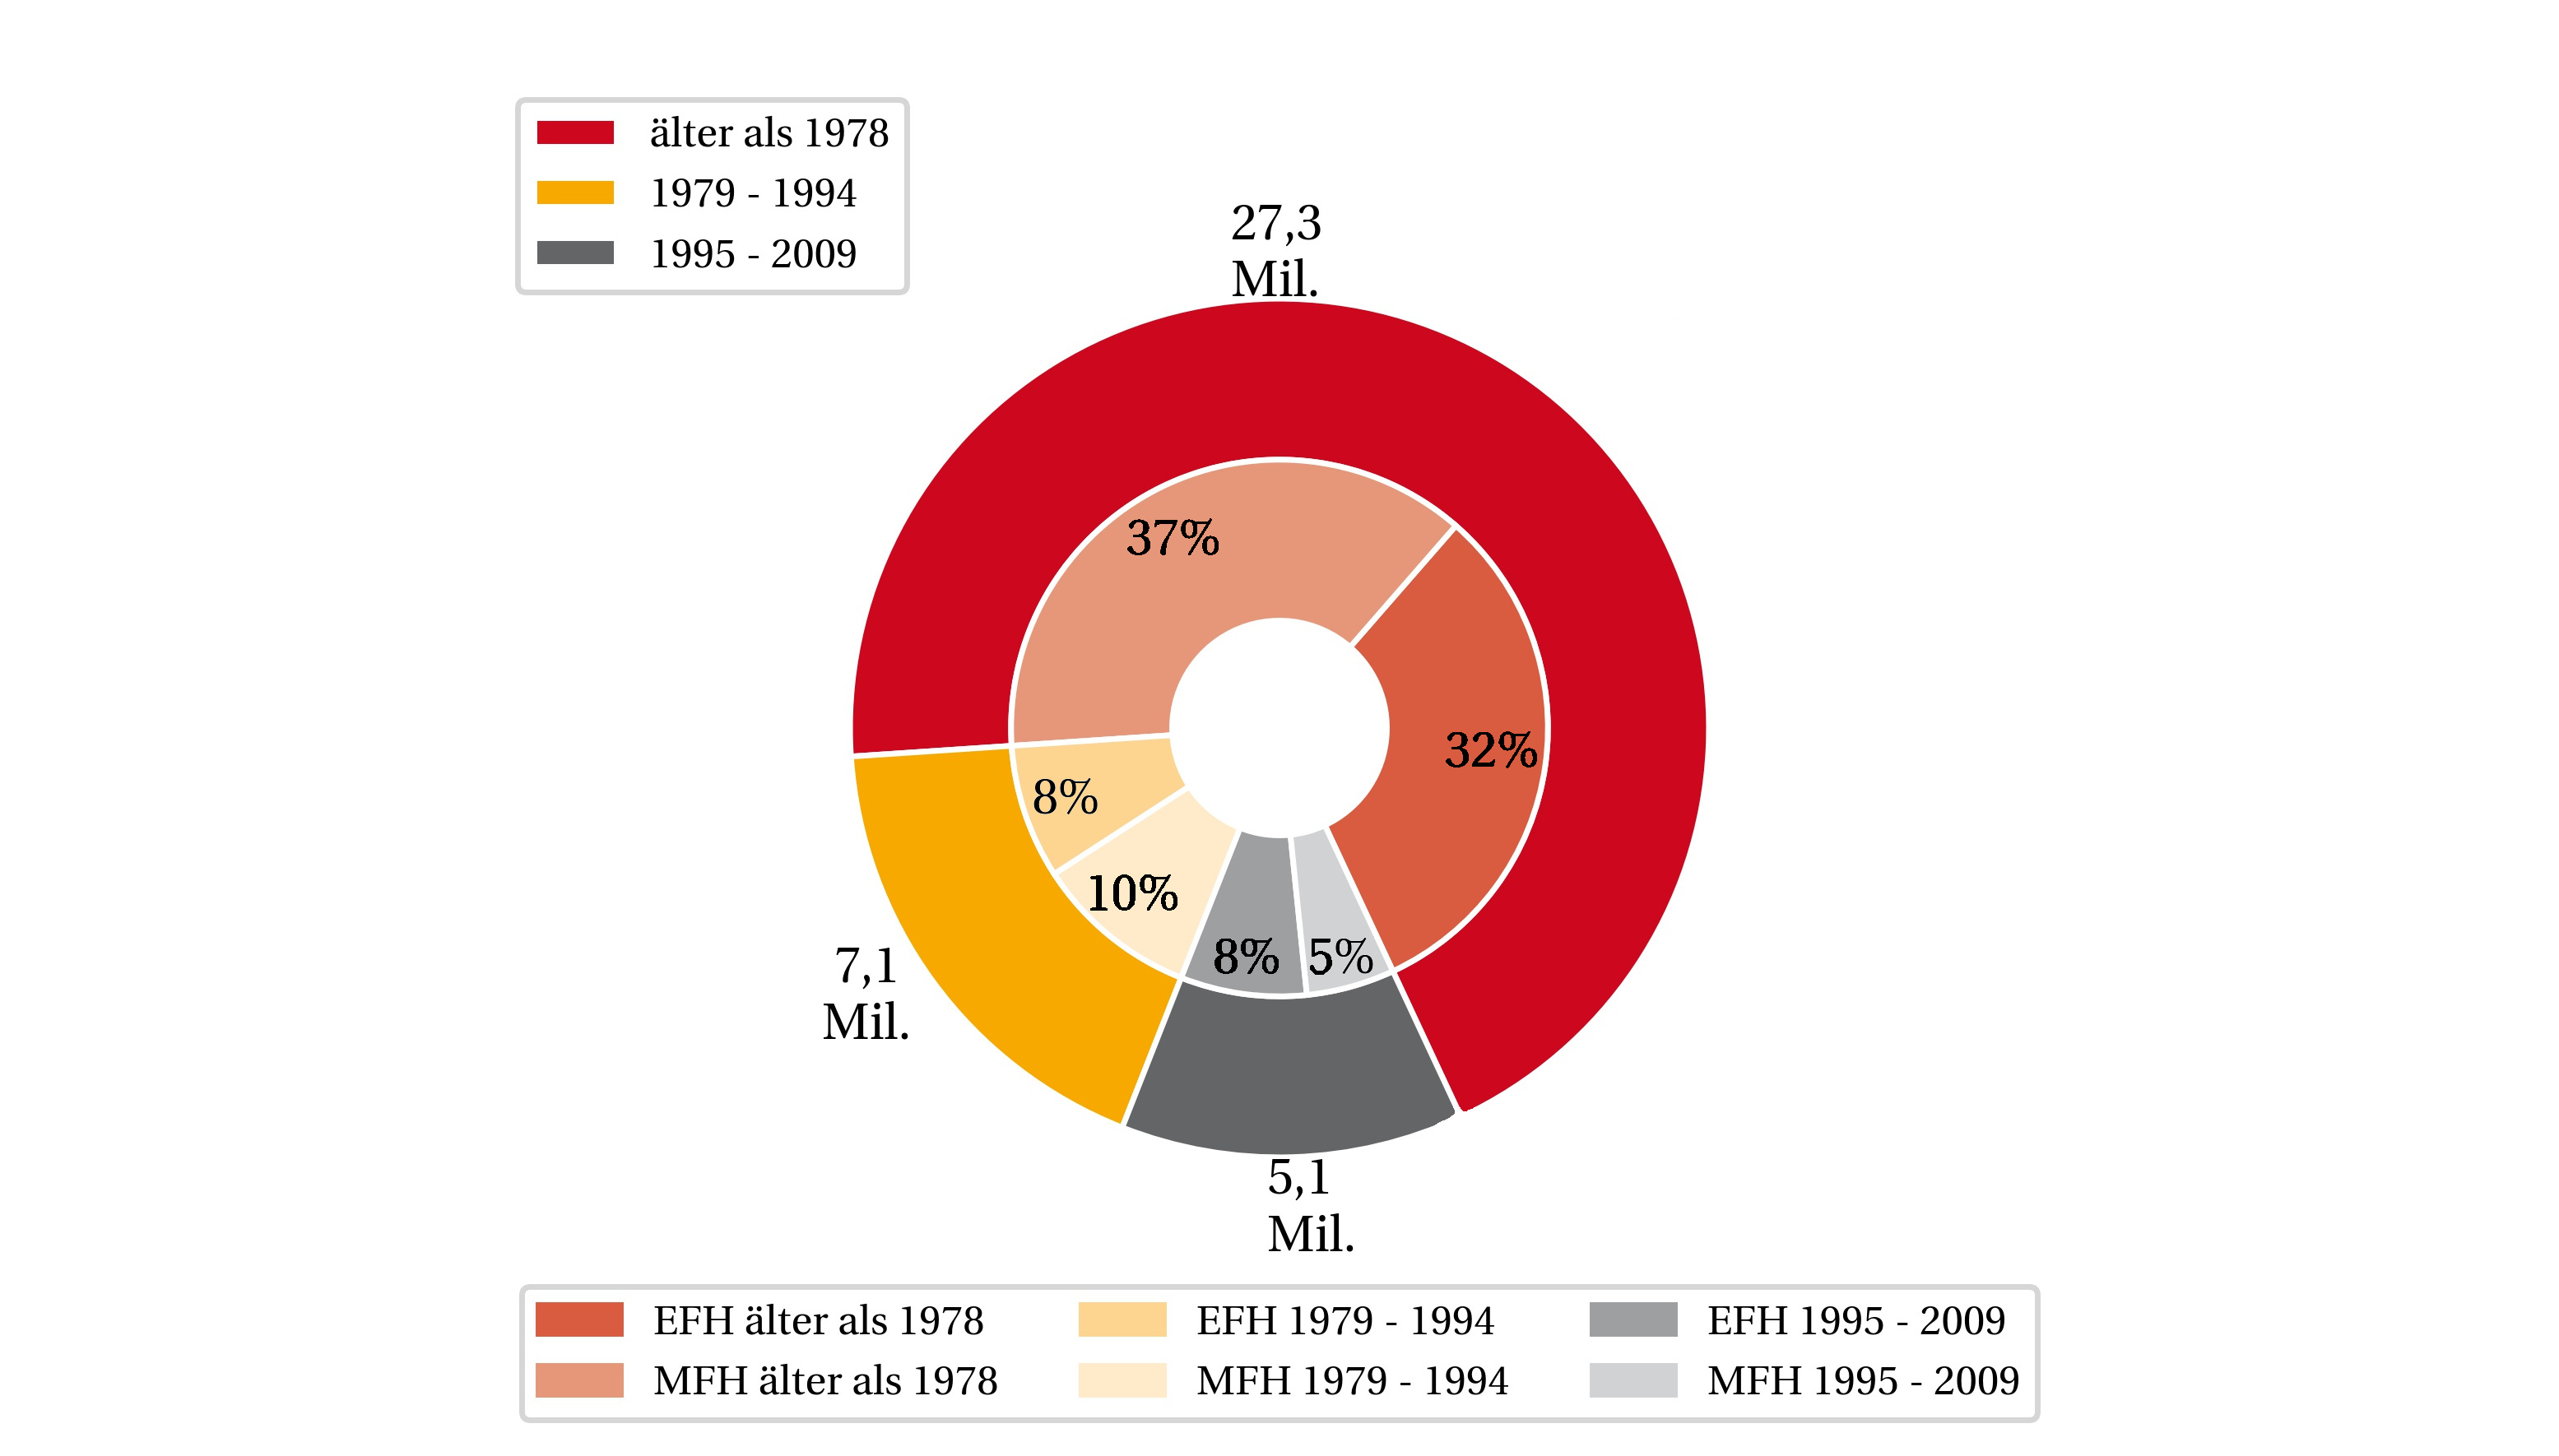
\includegraphics{Pictures/GebaeudeGroesse.jpg}
	\caption{Anzahl an Wohneinheiten bei Einfamilienhäuser (SFH) und Mehrfamilienhäuser (MFH) \cite{StatistischeAmterdesBundesundderLander.2014b}}
	\label{fig: Abbildung212} 
\end{figure}

Zusammenfassend lassen sich folgende Punkte bei der statistischen Betrachtung des deutschen Gebäudebestandes festhalten:

\begin{itemize}
	\item $\nicefrac{2}{3}$ aller Gebäude des Bestandes wurden vor der 1. Wärmeschutzverordnung 1978 errichtet.
	\item Ein- und Zweifamilienhäuser stellen mit 87\,\% den größten Anteil dar.
	\item Bei einer Betrachtung der Wohneinheiten teilt sich der Bestand in Gebäude mit einer oder zwei Wohnungen (47\,\%) und drei oder mehr Wohnungen (53\,\%) auf.
\end{itemize}

%Wohnobjekte?
%Zensus näher erläutern?
%Auf jeden Fall TABULA und Typgebäude näher beschreiben.
%Auf Wohnfläche eingehen?






\section{Historische Entwicklung der Dämmstandards}
\label{sec:Sektion 22}

Nachdem im vorherigen Kapitel der Gebäudebestand nach Alter und Größe beschrieben wurde, werden nun die zu den jeweiligen Gebäudealtern und -größten zugehörigen Dämmstandards vorgestellt. 
Hierzu wird zwischen der Isolierung verschiedener Gebäudebauteilen unterschieden. 
Neben Möglichkeiten zur Dämmung des Daches beziehungsweise der obersten Geschossdecke und der Außenwand werden zudem die Dämmung des Bodens sowie die Fenster betrachtet.
%Warum Dach und oberste Geschossdecke zusammengefasst werden kurz erklären?
%Näher auf Fenster drauf eingehen? Bzw. Fenster werden nicht gedämmt?

Ein wichtiger Kennwert zur energetischen Bewertung eines Gebäudes und einzelner Gebäudekomponenten beschreibt der U-Wert.
Hierbei handelt es sich um den Wärmeübergangskoeffizienten, welcher den Wärmestrom durch 1\,m² Bauteilfläche bei 1\,Kelvin Temperaturdifferenz beschreibt. 
Berechnet wird dieser als Kehrwert des Wärmedurchgangswiderstand \(R_T\). 
Der U-Wert ist definiert als
\begin{equation}
\label{eq:Gleichung221}
U = \frac{1}{R_T}  \ \ \ \ \ \ \ \text{in} \ \ W/(m^2 \cdot K)
\end{equation}
wobei mit
\begin{equation}
\label{eq:Gleichung222}
R_T = \sum \limits_{i} \frac{d_i}{\lambda_i}	
\end{equation}				%Muss ich da innere, äußere Schicht unterscheiden?
der Wärmedurchgangswiderstand als Verhältnis der Dämmstoffdicke \(d_i\) einer Dämmschicht \(i\) und der Wärmeleitfähigkeit \(\lambda_i\) des Baustoffes der Schicht \(i\) beschrieben wird. 

Für transparente Bauteile und somit explizit für Fenster variiert die Berechnung des Wärmedurchgangskoeffizienten \(U_w\):
\begin{equation}
\label{eq:Gleichung223}
U_w = \frac{A_g \cdot U_g + A_f \cdot U_f + l_g \cdot \psi_g}{A_g + A_f}  \ \ \ \ \ \ \ \text{in} \ \ W/(m^2 \cdot K)
\end{equation}
Hierbei beschreiben \(A_f\) den Flächenanteil des Fensterrahmens und \(A_g\) die Glasfläche. Ferner sind \(U_g\) und \(U_f\) die Wärmeübergangskoeffizienten der Verglasung (Index g) und des Fensterrahmens (Index f). 
Außerdem werden Wärmebrückenbildungen des Glasrandverbundes mit der Multiplikation des \(\psi\)-Wertes mit der Gesamtumfangsfläche der Verglasung \(l_g\) berücksichtigt. \cite{Laasch.2013}
%Wärmebrücken erklären?

Aus den Definitionen des U-Wertes und des Wärmedurchgangswiderstandes lässt sich leicht erkennen, dass die Wärmeverluste eines Gebäudes stark von der Dicke und den Dämmeigenschaften des Dämmmaterials abhängen. 
Hierbei lassen sich historische Unterscheidungen treffen.

Wie in \cite{.2015} dargelegt, werden die Gebäude mit Baujahr älter als 1919 von der Epoche der Gründerzeit geprägt.
Diese wird durch einen fortschreitenden Städtebau und den Beginn der Industrialisierung des Bauwesens charakterisiert. 
Aus wärmetechnischer Sicht lässt sich festhalten, dass es zu dieser Zeit kaum Regulationen bezüglich des Wärmeschutzes gab. 
Einzig die Dicke der Mauerschicht wurde mit 38\,cm empfohlen, wobei den Dämmstoffen geringe Relevanz zugeordnet wurde. 
Anstatt durch wärmetechnischen Maßnahmen an der Gebäudehülle Heizkosten zu senken, sparte man beim Bau und durch geringes Heizen. \cite{EickeHenning.2011}

Zwar kam es in dem Zeitraum von \mbox{1919 - 1948} zur zunehmenden Industrialisierung der Baustoffherstellung, allerdings blieb die zuvor genannte Mentalität des kostengünstigen Bauens anstelle von Maßnahmen zum Wärmeschutz erhalten. 
Auch nach Einführung der DIN 4110 \glqq Technische Bestimmungen zur Zulassung neuer Bauweisen\grqq\,behielt das Vollziegel-Mauerwerk mit 38\,cm Dicke den Stand als Standard im Hochbau. 
\cite{EickeHenning.2011}

Wie zuvor bereits kurz erläutert, beschreibt die Epoche von \mbox{1949 - 1957} die Nachkriegszeit mit ihrem schnellen Wiederaufbau. 
Signifikant für die Nachkriegsbauten, ist die Wiederverwertung von Trümmern. 
Die im Jahr 1952 eingeführte DIN 4108 verkörperte den ersten Ansatz Wärmeschutz normativ zu regulieren. 
Trotz deren Name \glqq Wärmeschutz im Hochbau\grqq \,beinhaltete die Norm nur einen Mindestwärmeschutz zur Vermeidung bauphysikalischer Schäden durch Schimmelbildung. 
Dadurch blieb die Nutzung von Dämmstoffen weiterhin die Ausnahme und es wurde auf das bewährte 38\,cm Mauerwerk zurückgegriffen.
Des Weiteren gab es bis dahin auch keine Normierung der Fenster, sodass hier ferner die Einfach-Verglasung die Konvention darstellte. \cite{EickeHenning.2011}
%Verglasung erläutern?
%Die drei Abschnitte in einen zusammenfassen?
%Zeitstrahl wäre nice

1958 - 1968: requirements on thermal insulation in force (DIN 4108 – "Wärmeschutz im Hochbau"); further industrialisation of building construction; development of panel buildings (GDR: "Plattenbauten")

1969 - 1978: new industrial building techniques (sandwich elements); also introduction of pre-fabricated single family houses (lightweight constructions "Fertighaus"); thermal insulation becomes more relevant in consequence of the first oil crisis

Nach der Ölkrise von 1974 rückte die Bedeutung des ressourcenschonenden Bauens beziehungsweise Betriebes von Gebäuden in den Vordergrund. 
Der Gesetzgeber verabschiedete am 11. August 1977 mit der 1. Wärmeschutzverordnung, im Folgenden mit 1. WschV abgekürzt, erstmalig eine Verordnung, in der ein Standard zur Minimierung des Heizwärmebedarfs festgelegt wurde. 
In Folge der 1. WschV verbesserte sich die Dämmeigenschaften der Bauten mit Baujahr \mbox{1979 - 1983}.
So lässt sich bei dem Tabula SFH-Typgebäude dieser Jahrgänge feststellen, dass sowohl das Dach eine 8\,cm Dämmung als auch der Boden eine 4\,cm dicke Dämmschicht besitzen. %(Vgl. Anhang? Zitat?)
Weiterhin wurde durch die Verordnung vorgeschrieben, dass \glqq außenliegende Fenster und Fenstertüren von beheizten Räumen (...) mindestens mit Isolier- und Doppelverglasung auszuführen (sind)\grqq \cite{Bundesregierung.1977}.
Somit ermöglichte die 1. WschV eine Verbesserung des energetischen Standards der Wohngebäuden. 
Allerdings stellten die ersten normativen Anforderungen an die Gebäudehülle aus heutiger Sicht nur einen Zwischenschritt hin zu einem energetisch sinnvollen Standard dar.
Als Beispiel hierfür ist die Anforderung an Fenster zu nennen. 
Für diese wurde in der 1. WschV festgelegt, dass ein U-Wert von 3,5\,\(W/(m^2 \cdot K) \) nicht überschritten werden darf \cite{Bundesregierung.1977}.
Nach heutigem Standard der Energieeinsparverordnung 2009, die im folgenden noch weiter erläutert wird, sind für die Fenster im Neubau \(U_w\)-Werte kleiner 1,3\,\(W/(m^2 \cdot K) \) einzuhalten.

1984 - 1994: 2nd thermal protection ordinance (2. Wärmeschutzverordnung); GDR: further improved insulation ("Rationalisierungsstufe III")
market introduction of low energy houses, supported by regional grant pro-grammes

1995 - 2001: 3rd thermal protection ordinance (3. Wärmeschutzverordnung); considera-tion of a bonus in the tax in case of realisation of a low energy house

2002 - 2009: energy saving ordinance ("EnEV 2002"), considering building and heat supply system; KfW grant programmes ("KFW-Energiesparhaus 60 and 40”, Passive Houses)

2010 ... : new requirements of energy saving ordinance ("EnEV 2009") on the level of low energy buildings
new KfW grant programme regulations ("KFW-Effizienzhaus 70, 55 and 40”, Passive Houses)

\begin{figure}[H]
	\centering
		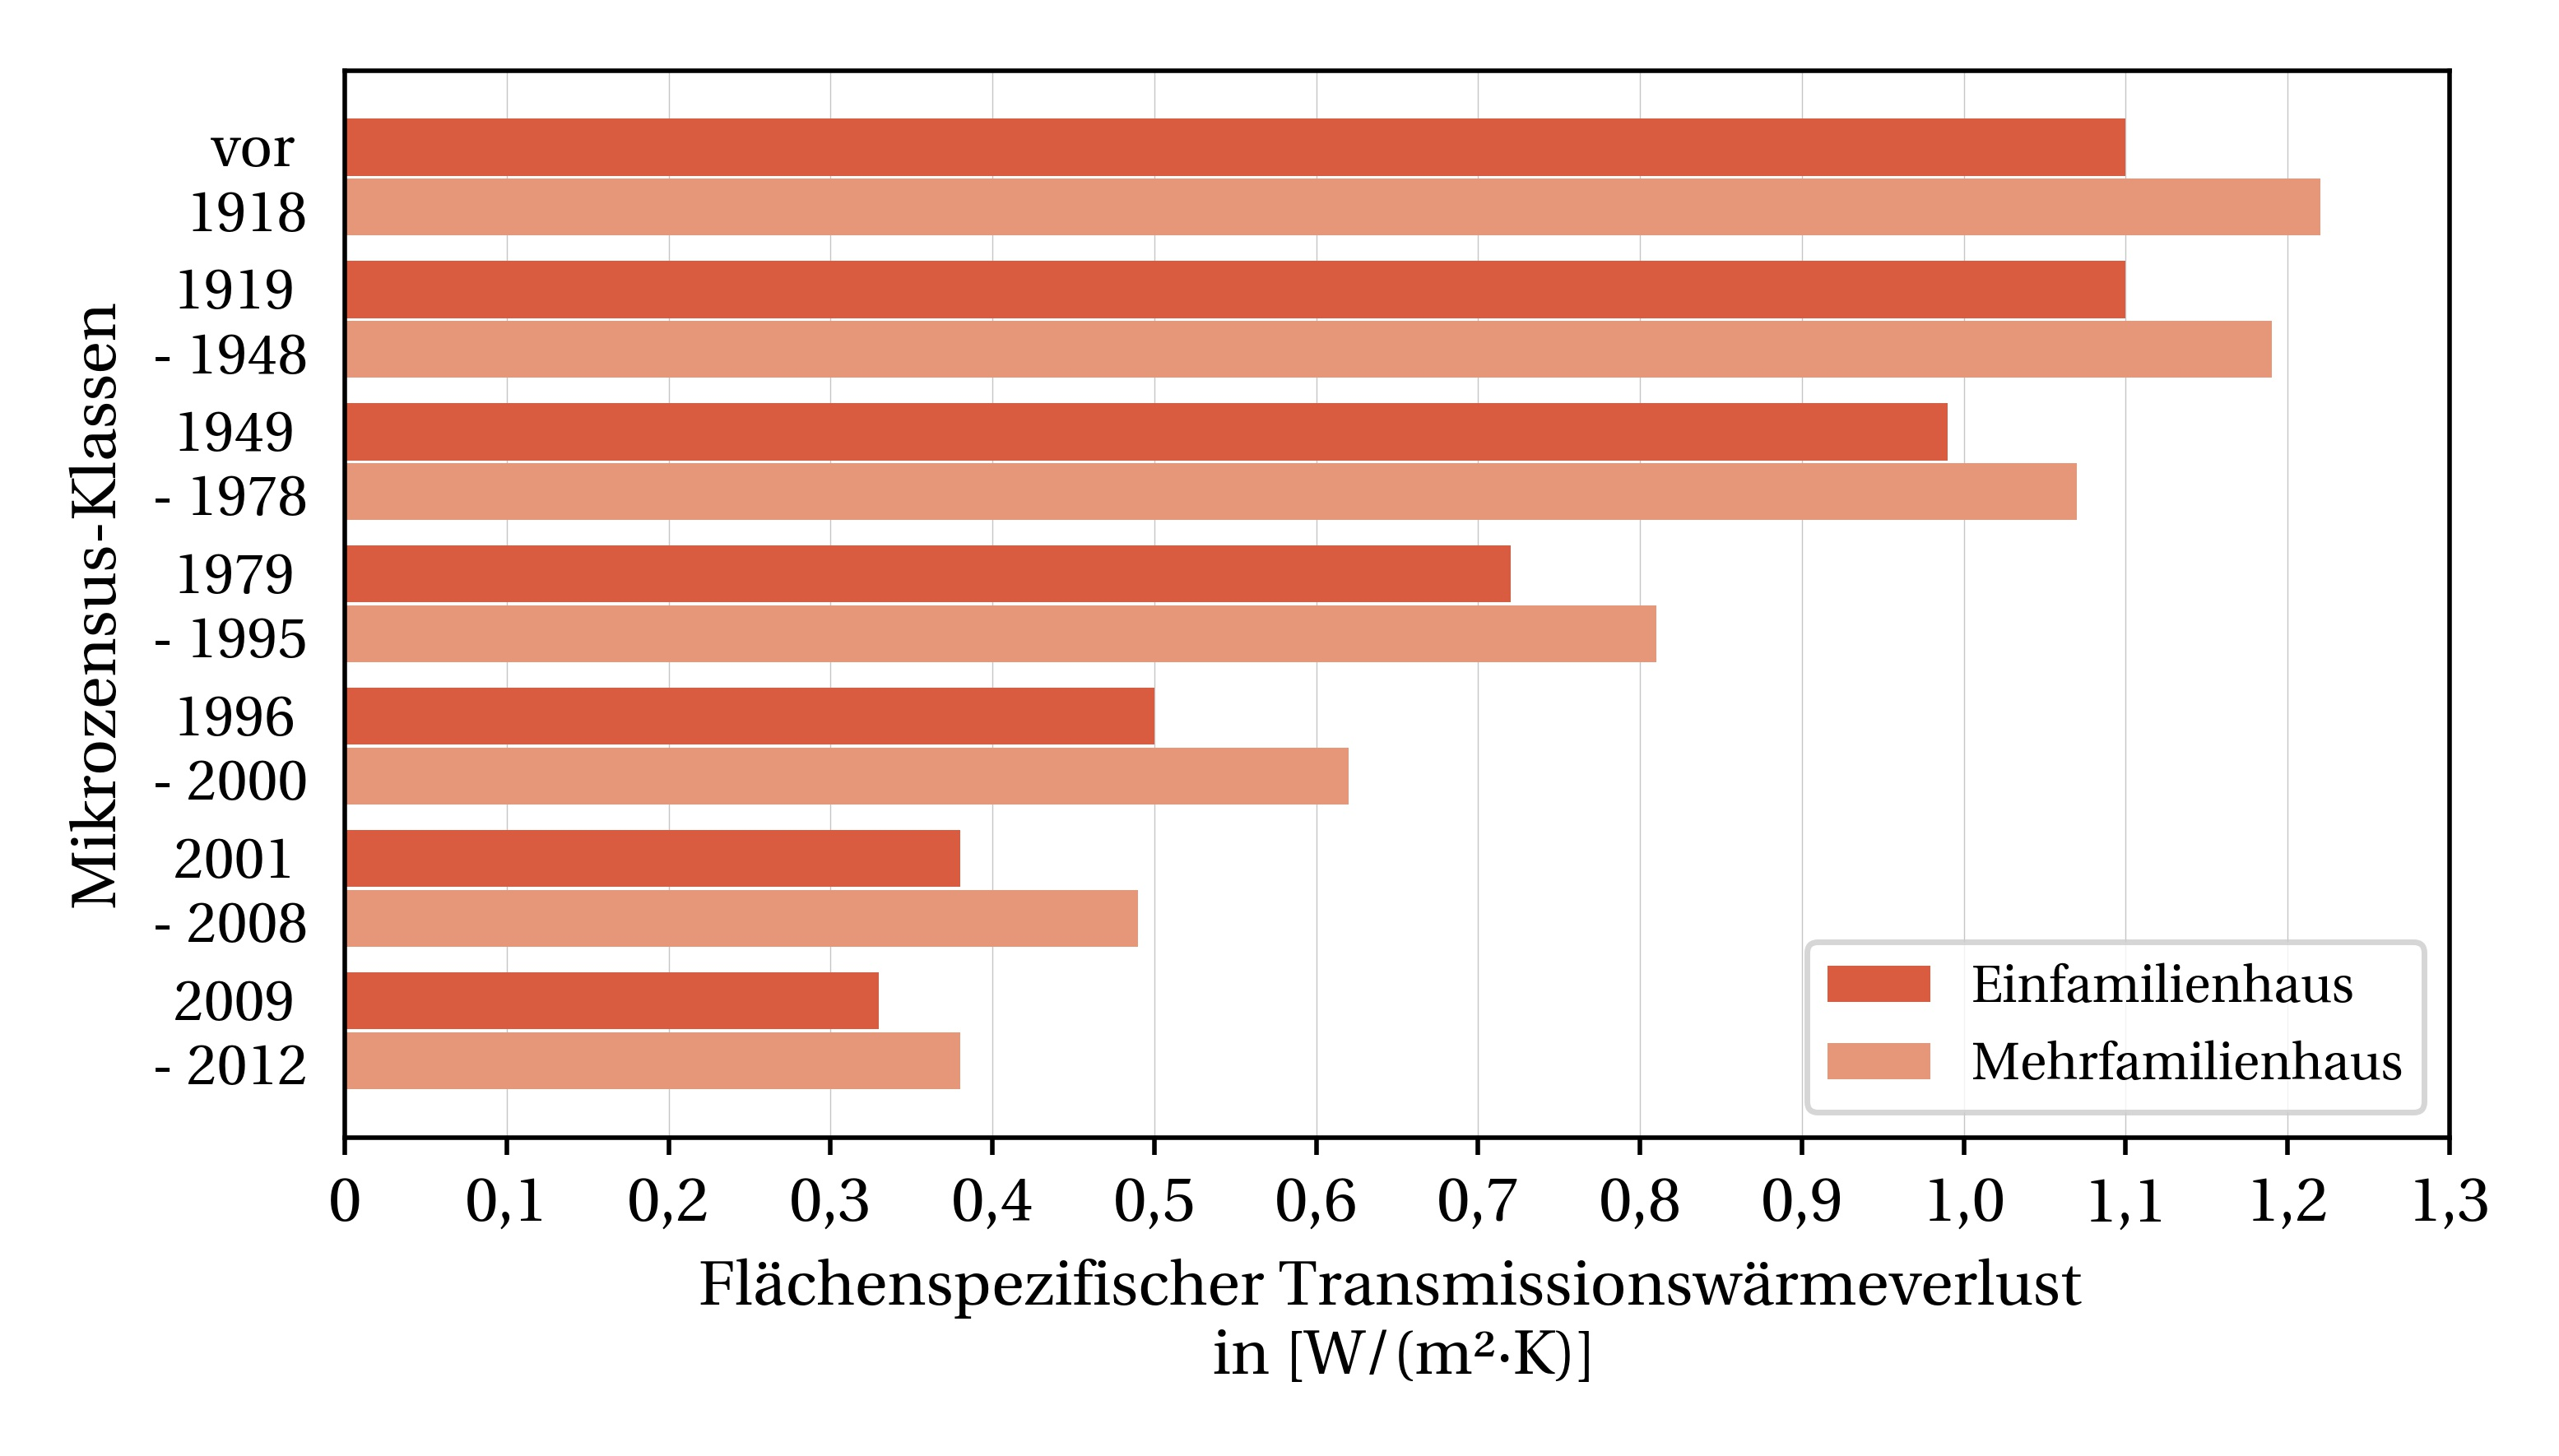
\includegraphics{Pictures/TransmissionswaermekoeffizientBaujahr.jpg}
	\caption{tba}
	\label{fig: Abbildung221} 
\end{figure}






\section{Sanierungsstand des deutschen Wohngebäudebestandes}
\label{sec:Sektion 23}

In dem vorangegangen Abschnitt wurde die Entwicklung des Dämmstandard vorgestellt. 
Hierbei wurde sich ausschließlich auf den Neubauzustand bei Fertigstellung des Gebäudes bezogen.
Dieses Kapitel soll nun die Veränderung aus energetischer Sicht des Gebäudebestandes durch Sanierung veranschaulichen.

Abbildung \ref{fig: Abbildung231} zeigt den Anteil der durch nachträgliche Wärmedämmung sanierten Bauteilfläche nach Bauteilen und Gebäudeart.
Zu erkennen ist der große Anteil an sanierter Dachfläche beziehungsweise obere Geschossdeckenfläche.
Dieser liegt für SFH und MFH annähernd gleich bei etwa 57\,\%.
Folglich wurde mehr als die Hälfte der Dachflächen im Altbau nachträglich gedämmt.
Einen leichten Unterschied zwischen den Gebäudearten ist bei den nachträglich sanierten Außenwänden zu beobachten. 
Bei diesem Bauteil wurden bei MFH etwas mehr als 31\,\% mit einer besseren Dämmung versehen, wohingegen es bei den SFH nur etwa ein Viertel waren.
Deutlich weniger Relevanz bei der nachträglichen Dämmung erhielt die Isolierung des Fußbodens beziehungsweise der Kellerdecke. 
Für diese Bauteile wurden bei beiden Gebäudearten nur circa 10\,\% mit einem besseren Wärmeschutz versehen. 

\begin{figure}[H]
	\centering
		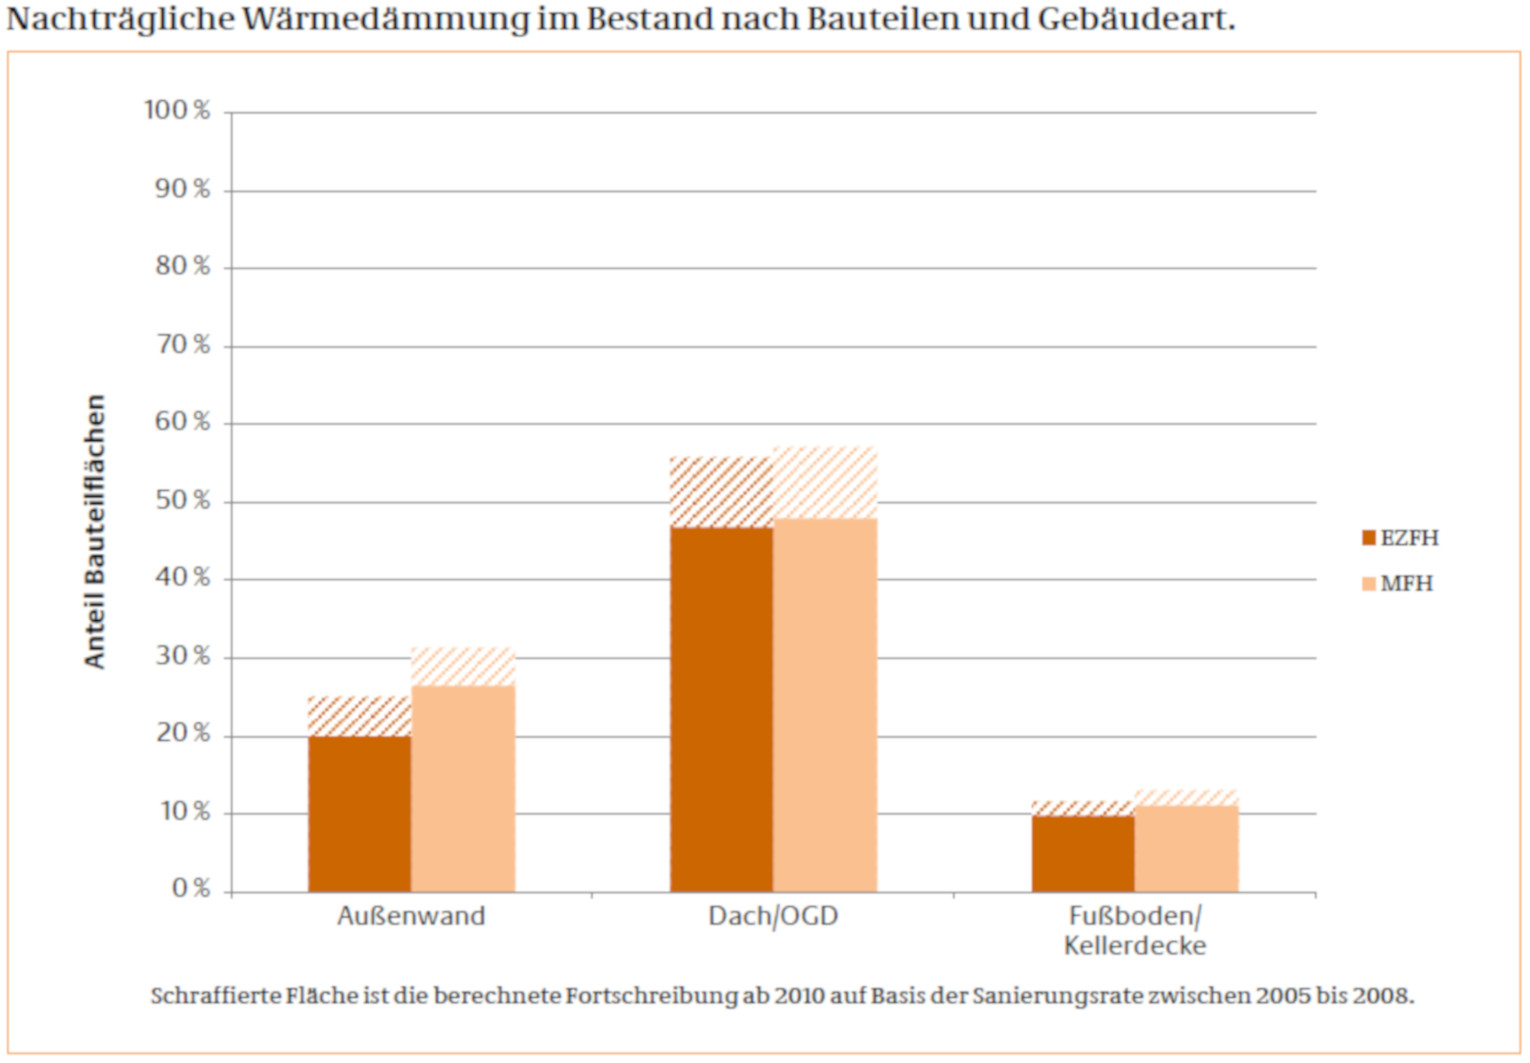
\includegraphics{Pictures/NachtraeglicheSanierung.jpg}
	\caption{\cite{Bigalke.2016}}
	\label{fig: Abbildung231} 
\end{figure}

In Abbildung \ref{fig: Abbildung231} fehlen die Angaben zum Sanierungsstandes der Fenster.
Hierfür ist die Datenlage der Sanierung schwierig, allerdings bietet \cite{Bigalke.2016} eine Schätzung über den Bestand an Fenstern im Jahre 2015.
Aus Tabelle \ref{tab: Tabelle231} sind verschiedene Verglasungsarten mit deren \(U_g\)-Wert sowie Anzahl und Anteil am gesamten Fensterbestand in Deutschland zu erkennen.
Wie in Gleichung \ref{eq:Gleichung223} dargelegt, beschreibt der \(U_g\)-Wert den Wärmedurchgang durch die Verglasung.

Obwohl die Einfachverglasung für einen großen Teil des Altbaues den Neubaustandard darstellte, ist deren Anteil am Fensterbestand mit nur noch 3\,\% sehr gering. 
%Aufgrund dessen enorm hohen Wärmedurchgangskoeffizient in Höhe von 5,8\,\(W/(m^2 \cdot K)\) ist die Rückläufigkeit dieser Fensterart als positiv zu bewerten.
Der heutige Bestand der Fenster wird durch unbeschichtetes Isolierglas sowie dem Zweischeiben-Wärmedämmglas dominiert, welche mit 34\,\% und 47\,\% vertreten sind.
Weiterhin ist zu erkennen, dass das Dreischeiben-Wärmeglas bereits 8\,\% des Fensterbestandes stellt, obwohl dieses erst 10 Jahren vor Erhebung der Daten auf den Markt kam.

\begin{table}[H]\centering
\begin{tabular}{lccc}
\toprule[1.5pt]
Verglasungstyp & Anzahl & Anteil am Bestand & \(U_g\)-Wert \\
 & [in Millionen] & [in \%] & [in \(W/(m^2 \cdot K)\)] \\ \addlinespace[5pt]
\midrule[2pt]
Einfachverglasung & 19,6 & 3 & 5,8 \\
\midrule
Verbund- und Kastenfenster & 44,8 & 7 & 2,8 \\
\midrule
Dreischeiben-Wärmedämmglas & 48,9 & 8 & 0,7 \\
\midrule
unbeschichtetes Isolierglas & 207,3 & 34 & 2,8 \\
\midrule
Zweischeiben-Wärmedämmglas & 284,2 & 47 & 1,4 - 1,1 \\
\bottomrule[1.5pt] \addlinespace[10pt]
\end{tabular}
\caption{Bestand an Fenstern in Deutschland, 2015 \cite{Bigalke.2016}}
\label{tab: Tabelle231}
\end{table}


\section{Optimierungsmodell}
\label{sec:Sektion 24}



